\documentclass[11pt]{article}
\usepackage{acl2016}
\usepackage[english]{babel}
\usepackage[utf8]{inputenc}
% \usepackage[numbers]{natbib}
% \usepackage{authordate1-4}
\usepackage{times}
\usepackage{url}
\usepackage{latexsym}
\usepackage{multirow}
\usepackage{todonotes}
\usepackage{newclude}
\usepackage{float}

% \def\op#1{\textcolor{red}{TODO\@ \textit{#1}}}

\def\op#1{\todo[linecolor=red,backgroundcolor=red!25,bordercolor=red]{#1}}

%% Compile with:
%% latexmk -pdf -interaction=nonstopmode -synctex=1 -pvc proposal.tex

%%%%%% PLEASE USE THIS DECLARATION FOR YOUR COMMENTS %%%%%%%%

% OP - Ondrej Platek inline 
\def\OP#1{{\color{purple}OP: \it #1}}
\def\ODdel#1{\bgroup\markoverwith{\textcolor{purple}{\rule[0.5ex]{2pt}{1pt}}}\ULon{#1}}

% OD - Ondrej Dusek
\definecolor{darkgreen}{rgb}{0.0, 0.5, 0.0}
\def\OD#1{{\color{darkgreen}OD: \it #1}}
\def\ODdel#1{\bgroup\markoverwith{\textcolor{darkgreen}{\rule[0.5ex]{2pt}{1pt}}}\ULon{#1}}


\aclfinalcopy% Uncomment this line for the final submission
%\def\aclpaperid{***} %  Enter the acl Paper ID here


\newcommand\BibTeX{B{\sc ib}\TeX}

\def\area#1{{\color{darkgreen}area:\it #1}}
\def\food#1#2{{Dial. state #1: \color{blue}food:\it #2}}
\def\pricerange#1{{\color{orange}pricerange:\it #1}}
\def\sys#1{{\color{purple}System: \it #1}}
\def\usr#1{{\color{brown}User: \it #1}}
\def\api#1{{\color{green}DB: \it #1}}

\title{Extracting Knowledge from Dialogue}

\author{Ondřej Plátek \\
  Charles University in Prague, Faculty of Mathematics and Physics \\
  Institute of Formal and Applied Linguistics \\
  Malostranské náměstí 25, 11800 Praha 1, Czech Republic\\
  {\tt oplatek@ufal.mff.cuni.cz}\\}

\date{}



\begin{document}
\maketitle
\begin{abstract}
Building a conversation agent is a demanding process which is typically simplified by using narrow fixed conversation domain.
The most effective approaches either use use a~very weak feedback and improve deployed dialog system or use supervised learning and labeled data.
This work build on the success of mentioned methods but focus on designing the conversational agents which will be able to:
\begin{itemize}
    \item collect explicit annotation interactively during the dialogue,
    \item enhancing the knowledge base of a system by new facts,
    \item learn explicit reward signals from conversations
\end{itemize}
Consequently, such conversational system should:
\begin{itemize}
    \item need smaller amount of data and annotation needed for its optimization 
    \item and self improve based on the collected feedback.
\end{itemize}
\end{abstract}

\section{Introduction}
\label{sec:introduction}
\todo{DESCRIBE MUCH THOROUGHLY MY FIRST EXPERIMENTS}
\todo{Explicit future section compare to the current state of the model}
\todo{Fix typos - obviously}
\todo{self-improving mention in introduction}
\todo{make clear that section 2 and 3 are others works}
\todo{Separate section experiments to Published, In progress, Future work}

The research of dialogue systems describes theories how interlocutors communicate, evaluates communication techniques for humans and artificial systems, and last but not least build the artificial conversational systems.
Arguably, the most understood and commercial successful artificial systems are conversation agents playing role of expert in task oriented dialogue in narrow domain.
Several research groups deployed such speech-to-speech on different domains, for example:
\begin{itemize}
    \item Let's go system~\cite{raux_lets_2005} helped the participants of experiments book a flight ticket.
    \item The Cambridge group repeatedly uses Cambridge restaurant domain to evaluate experiments on crowdsourced users where the user search for a restaurant in Cambridge.
    \item The work of~\cite{dusek_sequence2sequence_2016} and \cite{vejman_martin_development_2015} evaluates their system on Public Transformation domain in Prague and New York respectively on crowdsourced and also real users. 
\end{itemize}
All the mentioned works conclude that action selection the task of dialogue management plays central role in leading a dialogue.
However, the obvious differences between the domains and absence of widely accepted evaluation metrics for action selection do not allow comparison of the deployed techniques and algorithms.

The lack of comparable research was the reason for organizing dialogue state tracking challenge (DSTC)~\cite{dstcwilliams} which resulted in successful evaluation of many dialogue state trackers on the restaurant domain.
Dialogue state tracking probabilistically represents user's goal in predefined formalism such as dialogue acts~\cite{dstcwilliams,henderson2014second,hendersonthird} which is updated as the conversation evolves.
The~DST representation is evaluated by easy to understand and widely accepted measures such as accuracy and L2 measure.\footnote{DSTC2 and DSTC3 challenges recommend using accuracy and L2 measures. In addition, one is advised not to evaluate the dialogue state trackers on the first turns where the dialogue state does not change.}
The improvements of dialogue state trackers enable more informed and thus better action selection which is the ultimate goal of a dialogue system.

% Most of the dialog state trackers submitted to DSTC1, DSTC2 and DSTC3 used supervised learning to estimate the probabilities of dialogue state for given history\footnote{With the notable exception of~\cite{zilka_incremental_2015} tracker which perform simple Bayesian update without any learning and still achieves competitive results.}
As a result of the DST challenge success, the dialog state tracking specified by manually designed ontology was widely adopted as it was used in the DST challenges.
In general, we see the manually designed ontology as arbitrary, costly and also error prone process.\footnote{The Cambridge restaurant ontology was polished over several years of research and it is actually rather simple.}
Recently, it was shown by~\cite{wen_networkbased_2016} that the dialogue state annotations are the single annotations in additions to conversation transcriptions needed for training end-to-end system jointly, so it became even more important to specify high quality DST labels by the domain ontology.
In our recent work~\cite{platek2016wochat}, we proposed alternative annotations of dialogue history which we describe in~Section~\ref{sec:experiments}.

We draw another conclusion from the dialogue state challenge, that using n-best list from automatic speech recognition (ASR) helps just a little if compared with 1-best hypothesis even for ASR with high word error rates.
In addition, the recent advances in speech recognition reduced the WER even on far-field ASR drastically~\cite{peddinti_jhu_2015,zhang_highway_2016}.
As a result, we observed that the focus of the research moved to text-to-text systems which can be easily integrated to speech to speech systems using a~one-best ASR and a~text-to-speech (TTS) modules.

We see the following research goals in the field of dialogue systems as the most important to address in next five years:
\begin{enumerate}
    \item Reducing the number of data and annotation needed for deploying task-oriented dialogue systems.
    \item Exploiting feedback and learned knowledge from live interaction with users.
    \item Efficient exploiting knowledge gained from training a~single domain agent for extending its domain. 
\end{enumerate}


We propose a research direction which aims to tackle the first two problems, and if successful, it may help to solve also extending domain of the agent.

We review current state-of-the-art end-to-end dialogue system in Section~\ref{sec:e2end} in respect to our goals.
In Section~\ref{sec:learn_feedback}, we summarize how a feedback is used for optimizing statistical models and how it is represented and extracted. 
In Section~\ref{sec:experiments} we describe our results and we propose future work. 
Ideally, our experiments will show that proposed models are able to learn from user feedback and the resulting dialogue system will be able to self-learn.
Finally in Section~\ref{sec:discussion}, we review our work, discuss potential challenges and compare it to current research.


\section{End-to-End Conversational Agents}
\label{sec:e2end}
End-to-end conversation agents is a~new appealing approach for building conversation agents.
It reduces the task of building text-to-text dialogue system to training a single statistical model and thus which optimizes the response generation process jointly and thus avoid cumulating errors.

Neural networks dominate the first attempts~\cite{williams2016end,bordes_learning_2016,weston2015endtoend_prereq} to build conversational end-to-end systems.
Using neural networks is an obvious choice because different models achieve state-of-the-art results for optimizing traditional components of a dialogue system:
\begin{itemize}
    \item language understanding (LU) \cite{mairesse_spoken_2009} 
    \item dialogue state tracking (DST) \cite{williams_web-style_2014,henderson2014word,vodolan_hybrid_2015,platek_recurrent_2016}
    \item natural language generation (NLG) \cite{dusek_sequence2sequence_2016,wen_networkbased_2016}
    \item feedback/reward prediction~\cite{su_learning_2015}
\end{itemize}
Neural networks models not only achieve the best results in all the mentioned tasks but the models are relatively straightforward to combine and optimize jointly.
The key to successfully training a neural network is to provide enough labeled data for the neural network since it need to learn a lot of unspecified structure and patterns.
Luckily, neural networks capture structures in data latently so no annotation of the data structures is needed and one is able to collect data in much easier way.

\subsection{Data annotation and loss function}
\label{sub:data_annotation}

The supervised learning of neural networks suppose that one is maximizing directly the log likelihood of conditional distribution $ P(Y| X) $ where the parameters of the distribution are estimated from training samples $ (\hat{X}, \hat{Y}) $.
The sequential problems e.g.\ dialogue conversation are formulated as problem of generating next reply $y_t$ given the history $h_t$.
In case of dialogue system the history is represented by sequence of previous system utterances and user responses $ y_1, x_1, y_2, \dot x_{t-1}, y_{t-1}, x_t $.

Similarly to Hidden Markov Models (HMMs)~\cite{huang_hidden_1990} models Recurrent Neural Networks (RNNs) deal with potentially unlimited history by introducing a latent state $s_t$.\footnote{Unlike HMMs do not track probabilities in the hidden states but only sufficient statistics.}
Simple use of  RNNs~\cite{gers_learning_2000} for classification reminds the structure of HMMs for maximum likelihood estimation e.g.\ in ASR~\cite{huang_hidden_1990}, but RNNs model the observation probabilities discriminatively (see Figure~\ref{fig:encoder}).
The probability of action $ y_t $ is computed based on parameters for updating previous state $s_{t-1}$ to new state $s_t$ interpreting observation $x_t$.

\begin{figure}[htpb]
    \centering
    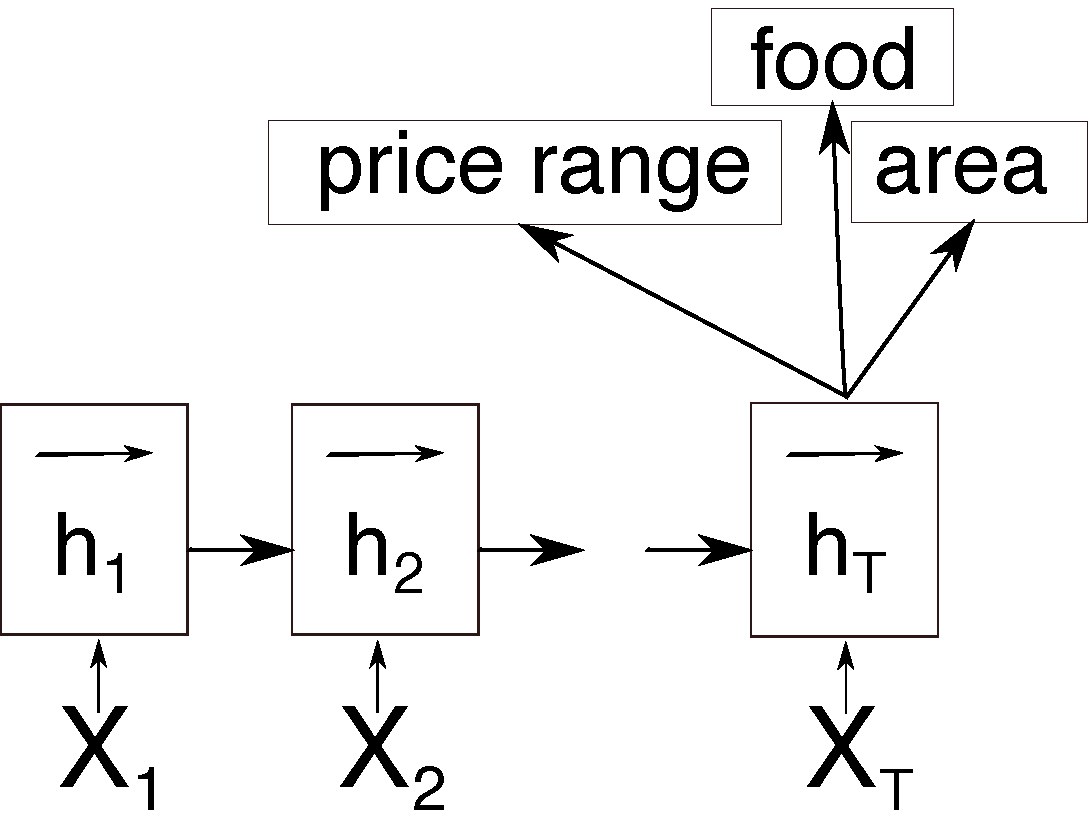
\includegraphics[width=0.8\linewidth]{encoder}
    \caption{RNN encoder for classification. The output variables are conditioned on the hidden state. This model was used as baseline in~\cite{platek_recurrent_2016} and it classifies classifies DST state slots based on the last hidden state $h_t$ independently.}
    \label{fig:encoder}
\end{figure}

In the work of~\cite{wen_networkbased_2016}, a neural end-to-end network model is trained for predicting dialogue history.
The model is not trained only from dialogue conversation and the domain DB but it uses annotations to speed up its learning.
Its dialogue history is expressed as $h_t = y_1, x_1, s_1, y_2, \dot x_{t-1}, y_{t-1}, s_{t-1}, x_t, s_t $ where $s_t$ is annotation of dialogue state in form of dialogue state items e.g {\it inform(food=Chinese, price\_range=expensive, area=west)}.
The work optimize the model using supervised learning by maximizing likelihood of next word in a reply using cross-entropy training.

The cross-entropy training is the most successful method how to train neural networks, but maximizing likelihood of next word in response should not be the ultimate goal which conversational agents should achieve.
First, supervised approaches are limited by quality of the golden data.
Second, the independence assumptions of generating next word from the hidden state are not true in dialogue.
Unfortunately, maximizing likelihood of the whole dialogue jointly is intractable because of data sparsity issues as there number of possible sequences of replies in dialogue grows very fast for more and longer dialogues.


\subsubsection*{Maximum likelihood: current state}\label{sub:maximum_likelihood}
Training neural networks for dialogue from gold labels using cross entropy for supervised learning brings several challenges
\begin{itemize}
    \item The prediction of the~next decision using the sequence-to-sequence model~\cite{bahdanau_neural_2014,sutskever_sequence_2014} are conditionally independent given the sufficient statistics of the hidden state of the decoding RNN.
    \item Dialogue responses of the system is often ambiguous and multiple options are equally possible.
        On the other hand cross-entropy models the same way uncertainty and ambiguity and allows only one correct gold solution.
        See Equation~\ref{eq:cross} where $p(x)$ is distribution approximated by distribution of samples over training data and updates of the neural networks needs to be perform only as difference between predicted likelihood $-log(q(x))$ and one log one-hot distribution
        \begin{equation}\label{eq:cross}
            H(p, q) = \sum_{x}{p(x) * (- log q(x))}     
        \end{equation}
    \item Further annotations of training pairs are costly and much more data is needed when annotations e.g.\ of dialogue state are not provided.
\end{itemize}

\subsubsection*{Weak supervision for reinforcement learning}\label{sub:batch_rl}

In this section, we introduce reinforcement learning (RL) as tool of our choice for optimizing the evaluation/reward/loss function e.g.\ user satisfaction or mimicking the whole dialogue.
Reinforcement learning is appealing approach for updating statistical model parameters when a feedback for action the system is delayed or noisy~\cite{williams2016end,bahdanau_actor-critic_2016,wierstra_recurrent_2010}.
In the field of dialogue systems, the RL was successfully used to optimize parameters of Gaussian processes used for selecting among several dozens of action~\cite{gasic2011line}.
On the other hand, using quite noisy feedback from thousands of live conversation with user feedback at the end of dialogues is not convenient for training neural networks because they need to update large number of parameters and such feedback is too weak.

Note RL was successfully used with supervised cross-entropy pre-training an later optimizing for not differentiable loss function.~\cite{williams2016end}
On the other, this approach still uses the same labeled data and annotations as used for supervised learning.
The advantage of this approach is that it is able to naturally capture by the reward functions multiple valid actions.
Furthermore, multiple weak reward functions can be combined to form much stronger feedback signal~\cite{abbeel_apprenticeship_2004}.

Reinforcement learning performance quality depends on the reward information which can be used for updating parameters of the model and also on the amount of data available.
Typically the reward is also used as scoring function for evaluating dialogues.
However, if using the scoring function as reward function for reinforcement one would like to automate the computation, but only partial and not satisfactory automatic scoring functions were suggested~\cite{liu_how_2016,lowe_evaluation_2016} so far. 
Note also that some RL algorithms such as Sarsa need are on-policy algorithms and need to used on life systems, we focus on algorithms which can be used also in off-policy settings~\cite{sutton_reinforcement_1998}.

\subsubsection*{Learning to collect feedback}\label{sub:irl}
If using the reinforcement or supervised learning it is assumed that the loss function is provided before the training.
One of key properties of dialogues systems is that their domain change over time~\cite{yu_evolvable_2016}, so every predefined loss function becomes obsolete after some time.
In addition, specifying a good loss is notoriously hard since no standard measures for dialogue are widely accepted.

Inverse reinforcement learning (IRL)\footnote{Also known as active reward learning~\cite{su2016active}.} is a task of learning the loss (or reward) function used in RL~\cite{abbeel_apprenticeship_2004}.
IRL could be used for learning how to interpret user feedback, but the IRL is ill-posed problem in general~\cite{choi_inverse_2011} and is guaranteed to work only for special cases e.g.~\cite{abbeel_apprenticeship_2004,choi_inverse_2011}.  \todo{Understand choi better}
In our experiments (see~Section~\ref{sec:experiments}) we aim to learn feedback from interactive conversation, but we plan to use IRL and similar approaches as reward shaping~\cite{su2016active} only for comparison.
We describe our approach of collecting explicit annotation in Section~\ref{sec:learn_feedback}.

Note, that collecting feedback explicitly for later use and IRL is not mutually exclusive.
Promising framework which may overcome vagueness of current system are adversarial networks especially~\cite{dumoulin_adversarially_2016}.
The adversarially learned inference (ALI) model is a deep directed generative model which jointly learns a generation network and an inference network using an adversarial process. 
The core idea is that one trains a generative model for dialogue system operator together with discriminator which attempts to recognize if generated dialogue is from the trained system or data sample from human (see Figure~\ref{fig:gan}).
We hope that discriminator may learn to distinguish the responses also on semantic level of the system's domain which current approaches mostly ignore. 

\begin{figure}[htpb]
    \centering
    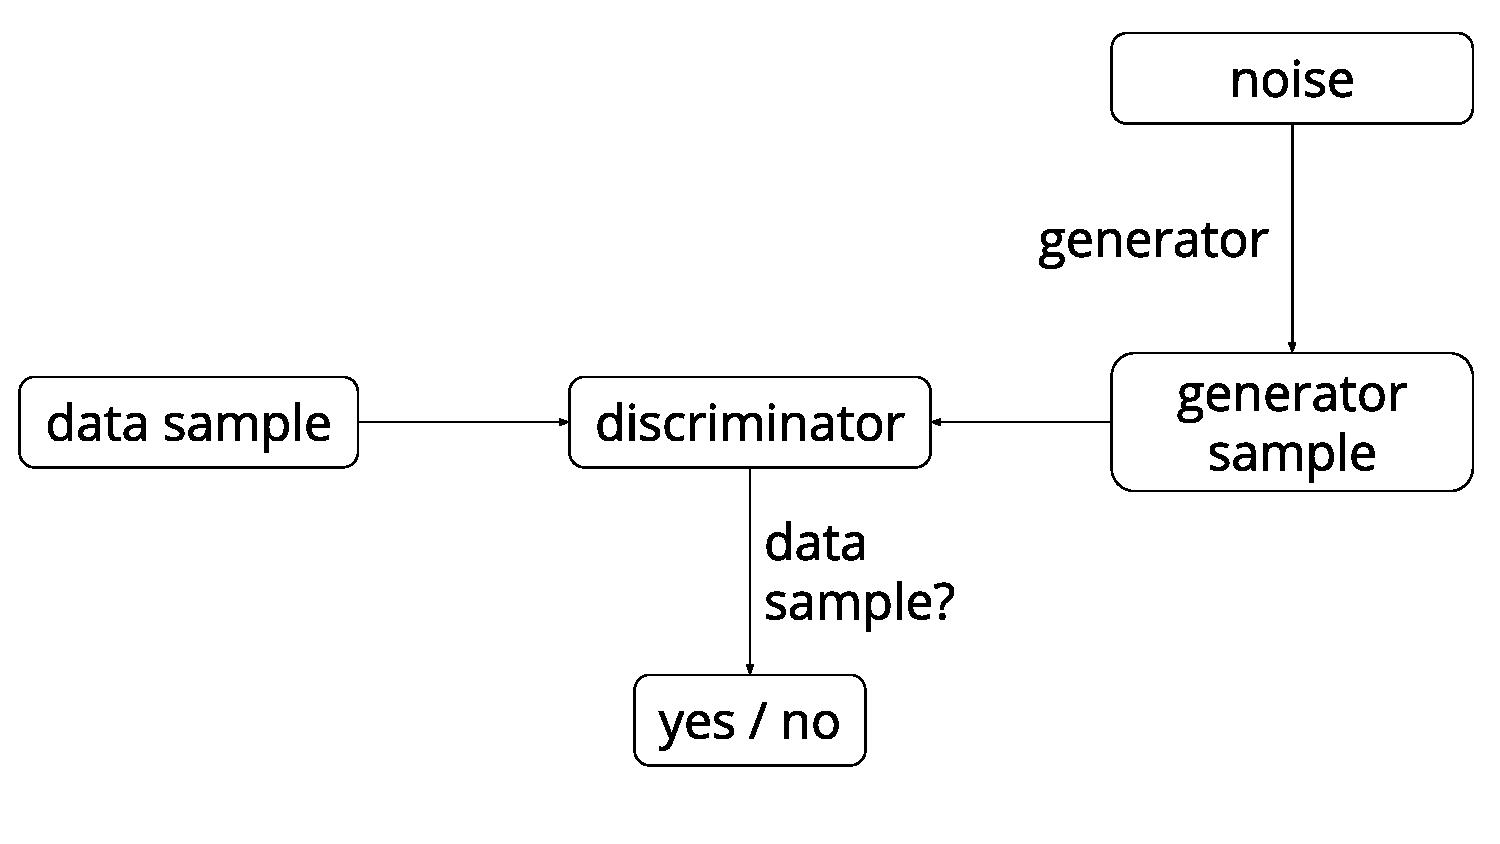
\includegraphics[width=0.8\linewidth]{gan_simple}
    \caption{Adversarial Learned Inference core idea~\cite{dumoulin_adversarially_2016}.\footnote{Picture taken from \url{https://ishmaelbelghazi.github.io/ALI/} website.} is to train of discriminator and generator as one network with two objectives. Discriminator separates real samples and generated samples and generator produce such artificial samples so that the discriminator cannot distinguish them from the real once.}
    \label{fig:gan}
\end{figure}

We are also interested in this approach because one should be able to see which positive examples contributed the most for the performance of the generator (the dialogue system) by exploring the error updates and performance of the discriminator.
Thus the discriminator could provide us with automatic annotations. 

\subsection{Architectures for neural end-to-end dialogue systems}
\label{sub:nn_architectures}
Neural architectures are used in two use-cases of conversational agents;
\begin{itemize}
    \item Chatbots - Such systems are learned without any structured knowledge from plain conversations.
    \item Task oriented system - learn to play role of expert and provides information from database to users.
        They are trained in respect to the specific content of their database.
\end{itemize}

The work of~\cite{serban_multiresolution_2016} is an example of neural network architecture which is able to mimic human-to-human conversations however quite often fails at capturing its semantics.
This line of research improves upon language modeling using neural networks~\cite{mikolov_efficient_2013} and adapts modeling of next word prediction by more efficiently representing the discourse structures.
The training of such models requires large corpora such as~\cite{lowe_ubuntu_2015}. 

On the other hand, the task-oriented dialogue system works attempt to extract the common knowledge in the dialogue with help of database containing domain related information.
A limited domain implicates that one is able to use only limited amount of data for training the systems.
The true challenge poses how to model access to the system calls to the database because the calls are not recorded in the data if plain text transcriptions of the dialogue are used.
One can only deduce that a part of the response is a result from some database call.

The work of~\cite{wen_networkbased_2016} solved the problem by using the annotation of dialogue state which determines database calls and corresponding natural language response convenient for given dialogue state. 
The simplistic system~\cite{williams2016end} showed that it is possible to use API calls\footnote{The system performs also other actions than accessed database so the term API call is used instead of DB calls.} without dialogue state annotation, but the system required {\it action mask} heuristics which determined whether an action is possible for given dialogue context.

\section{Collecting Feedback}
\label{sec:learn_feedback}
Extracting feedback from dialogues is possible in several ways as described earlier: through fixed loss function, through learned loss function or explicitly through annotations.
The feedback can be stored either explicitly as annotations or in parameters of the model which models the conversations.
We aim at learning to collect explicit annotations because annotations.
We focus on collecting explicit feedback because it can be exploited by any model via supervised or reinforcement learning in contrast to storing the feedback in parameters of a statistical model e.g.\ neural networks which notoriously hard to reuse for new architectures~\cite{oquab_learning_2014}.
We will also attempt to learn the feedback automatically because otherwise non trivial expert work is needed for designing the heuristics to collect the annotations.

\section{Experiments} \label{sec:experiments}

Our work focuses on building an end-to-end conversation agent which eliminates laborious handcrafting but needs significant amount of training. 
Our approach is does not only optimize action selection process of dialogue system, but also attempts to learn new facts and thus perform more informed decisions.
By introducing an end-to-end system that collects annotations which is used for its retraining we aim at reducing both the expert work and annotated data needed for launching such agent.
At the same time, such agent improves its performance by live interactions with users and the annotations may be helpful for adapting to a new domain.


We suggest following experiments to explore the crucial problems which need to be solved before a conversational agent is able to extract information through interaction and later used them for self improvement.
The experiments are designed as a proof of concept on narrow domain and scaling up to larger or multiple domains is left for future work or as obvious extensions. 

We first describe our published works, then we introduce work in progress and finally we propose future work. 

\subsection{Published work}
Our worked so far focused on developing an end-to-end task-oriented conversation agent on restaurant domain which is easy to train and provides reasonable baseline.
First, in work~\cite{platek_recurrent_2016} we verified that we are able to train recurrent neural networks for dialogue state tracking and achieve near state-of-the-art easily. 
We frame the DST as sequence-to-sequence problem and used encoder-decoder (see Figure~\ref{fig:dst_seq2seq}. 

\begin{table*}[tb]\vspace{-1mm}
\begin{center}
\begin{tabular}{l@{\quad}rll}
\hline
Model & Dev set & Test set\\
[2pt] \hline\rule{0pt}{12pt}
% Joint  &  todo &  todo \\
    Indep  &   0.892 & 0.727 \\
\hline
    \cite{vodolan_hybrid_2015} & - & 0.745 \\
    \cite{zilka_incremental_2015} & 0.69 & 0.72 \\
    \cite{henderson2013deep} & - & 0.737 \\
\hline
    DSTC2 stacking ensemble~\cite{henderson2014second} & - & 0.789 \\
\hline
\end{tabular}
\caption{Accuracy of our DST encoder-decoder compared to other implementation. The first group contains our systems which use ASR output as input, the second group lists systems using also ASR hypothesis as input. The third group shows the results for ensemble model using ASR output and also live language understanding annotations.}
\end{center}
\label{tab:dstc}
\end{table*}

\begin{figure}[htpb]
    \centering
    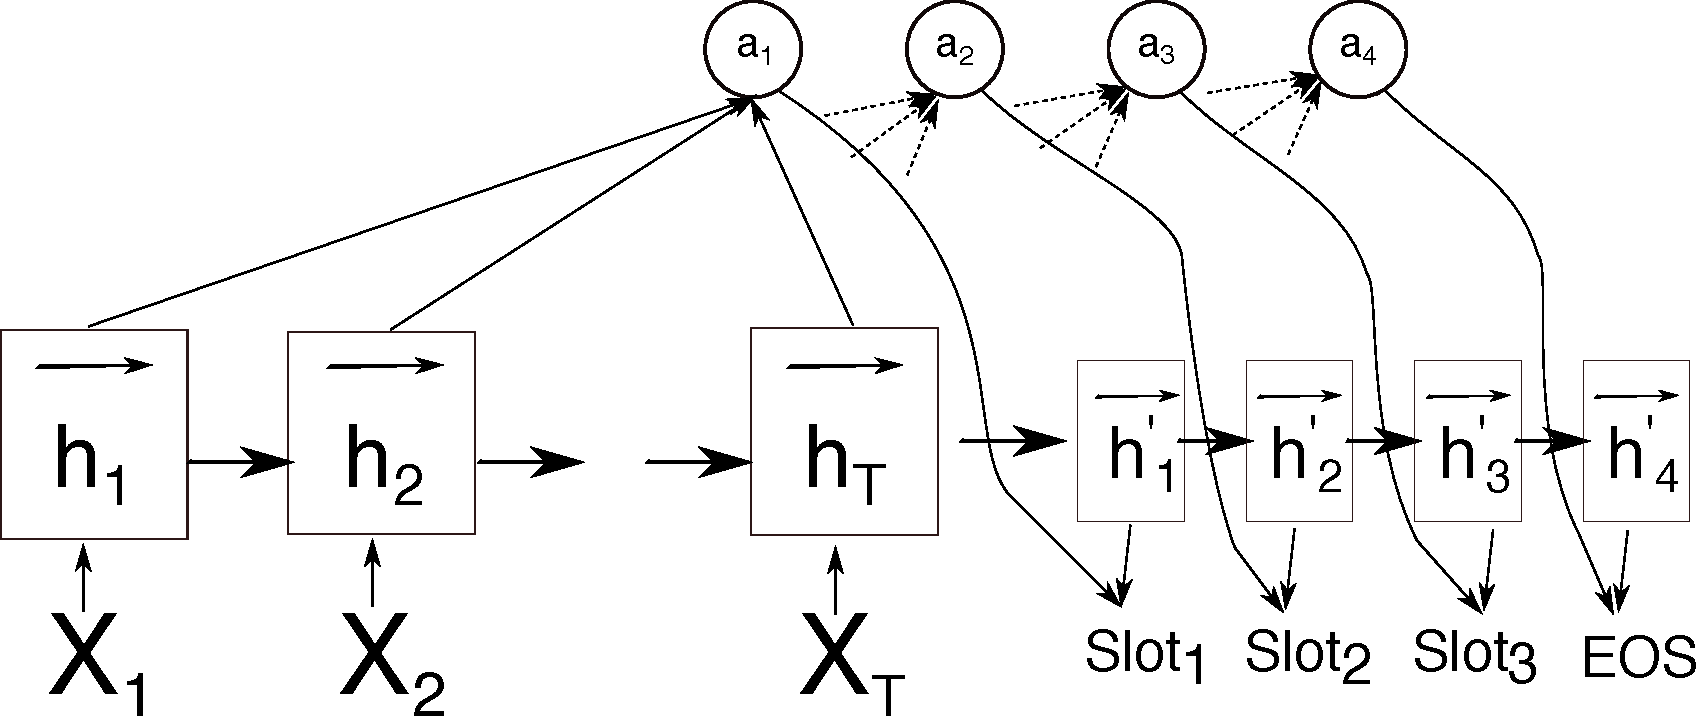
\includegraphics[width=1.0\linewidth]{dst_seq2seq}
    \caption{DST using encoder decoder RNN model.}
    \label{fig:dst_seq2seq}
\end{figure}

Second, a dataset for training end-to-end system~\cite{platek2016wochat} was collected which focus on collecting easy-to-obtained annotations.

\subsection{Work in progress}
We are still working on end-to-end system which can be optimized jointly.
In contrast, with very recent papers our approach will need much less annotation and won't use dialogue state labels as in~\cite{wen_networkbased_2016}, but DB calls as described earlier.

A crucial problem of statistically modelling a dialogue system in end-to-end manner is that the agent performs latent actions which from the conversation point of view appear rather stochastically due to lack of data.
However, the actions in fact follow strict logic.
Example of such (partially) latent actions are calls to database.\footnote{Any action of an agent can be transformed to operation on database from the dialogue system point of view because the dialogue system may delegate the task through the database to other services which execute the actions.}
If a system is supposed to query database for information it is a partially latent action because the system presents the results of the action to user.
However, the user can not distinguish if the system is providing similar answer without accessing the database e.g.~choosing a~reasonable but incorrect answer based on the language model.
An example of completely latent action is if a user request a Pizza the system should access the database and create and entry to database.
However, the user typically only suppose that the system executed the correct action.
As a result if one want to train a dialogue system one need to design objective function and data representations which force the latent action correspond to system replies, so the logic of the latent actions is maintained.

A common approach is to use dialog state tracking for updating the dialogue state represented in discrete form such as dialogue state items (see Figure~\ref{fig:dai_gen}) and a dialogue policy which execute operations on KB and produces plan for NLG what to say which is compatible with KB actions~\cite{dusek_sequence2sequence_2016,young2010hidden}.
Alternative approach is presented in simplistic form in~\cite{wen_networkbased_2016} where a KB operation is executed or skipped based on the dialogue state but the NLG uses the only the dialogue state and the result of KB operation to generate reply.
We propose to predict directly which KB operation to use from hidden state $h_t$ of neural network and based on the select KB operation's result and the same state $h_t$ predict sequence of words what to reply.
Such model needs to be trained to match KB actions and its replies but allows flexibility how to communicate about system actions which is goal of our research.
\todo{describe the model in detail}
\todo{describe expected results}

\begin{figure}[htpb]
    \centering
    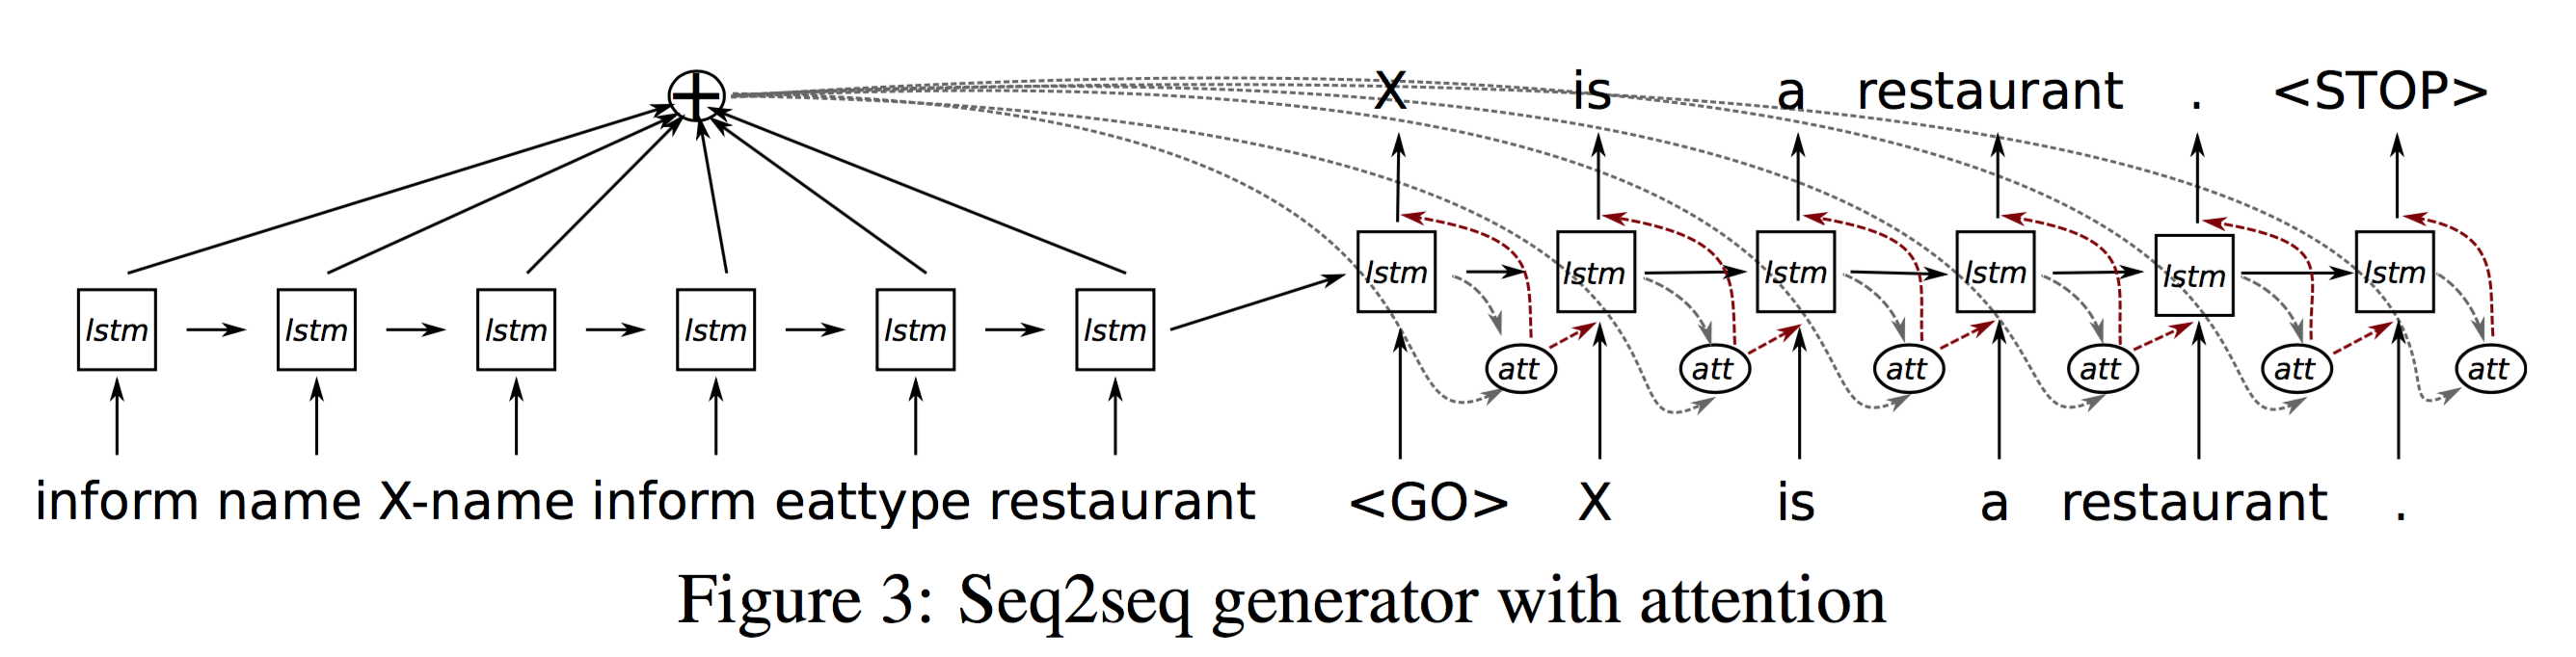
\includegraphics[width=1.0\linewidth]{dusek_seq2seq}
    \caption{Dialogue act items tracking and generation. A policy ensures that each access to DB corresponds to NLG plan what to say~\cite{dusek_sequence2sequence_2016}.}
    \label{fig:dai_gen}
\end{figure}

\subsection{Future work}

\subsubsection*{Easy first decoding for dialogue state tracking using reinforce algorithm}
We show in work~\cite{platek_recurrent_2016} that modeling DST as sequence-to-sequence may captures correlation between dialogue state values and also does nut suffer much from data sparsity.
However, the order dialog state labels is arbitrary chosen and may not be optimal for prediction dialogue state.
In this experiment, we rephrase the DST task as sequence-to-set model by employing loss function which prefers if three hypotheses labels match the set of gold labels $\{food\_type, area, price\_range\}_{hypotheses} = \{food\_type, area, price\_range\}_{gold}$.
Such loss function is in sharp contrast with combined cross-entropy loss maximizing probability true labels in order food, area and price range.
The sequence-to-set loss function is not smooth and cannot be differentiated, but we will use reinforce algorithm~\cite{williams_simple_1992} to update the model parameters.
We plan to pre-trained the model with cross-entropy updates and later fine tuned the weights with reinforce training.
% We do not plan to use the reinforce algorithm for tis less stable if one try to use larger steps size e.g. by AdaDelta algorithm~\cite{adadelta} as used for cross-entropy training.
Given the same model and the same number of parameters we expect the model trained with reinforce algorithm to perform better than cross-entropy training with early stopping because we will directly optimize the evaluation function.
In addition, it will be interesting to explore which permutation of slots is best to use for DSTC2 dataset and if the best permutation differs for each dialogue.
Using the reinforce algorithm on well pre-trained model we want to examine if easy-first decoding of slots can perform better than arbitrary chosen order of predictions. 

\subsubsection*{Discovering hidden database calls}
The dialogue system generates two kinds of actions; responses and calls to database.
The calls to the database influence the system replies in future turns by presenting their results or by changing results of next database calls.
This experiment focuses on such DB calls which results are at least partially presented to the user in the next reply.

Even if the DB results are immediately presented the database operations are not obvious.  
The first example in Figure~\ref{fig:apicall} demonstrates that the system presents one of possible results of the DB call to the user.
In the second example, the system replies the single possible answer {\it in the west part} to the query {\it select restaurant.area where name="India house"}.
However, in the second example the same result can be obtained by many similar queries where name is replaced by $x=\{travellers\ rest, la\ margherita, \ldots\}$ in query {\it select restaurant.area where name="$x$"}.
We formulate the task as a classification problem where the classifier assign high probability to DB calls which are able to produce results compatible with the system reply and ideally the highest probability should be given the DB call intended by the user.

The evaluation criteria for experiment are if the system replied with valid property and if the DB call used the property from entity which is valid given the history.
We plan to use for evaluation the dataset collected in work~\cite{platek2016wochat} where if the entity is valid given the history the DB call is unambiguous. 

\begin{figure}
    \dots \\
    \usr{I would like a Chinese restaurant} \\
    \sys{In which area?} \\
    \usr{In the city center} \\
    \api{select restaurant.name where area="city center" and food="Chinese"}
    \sys{A golden house is a Chinese restaurant in the city center} 

    \dots \\
    \usr{Where is of the India house restaurant located?}
    \api{select restaurant.area where name="India house"}
    \sys{The India house is located in the west part of the city.}
    \caption{Dialogue example with latent calls to system's DB.}
    \label{fig:apicall}
\end{figure}


\subsubsection*{End-to-end system for consistent DB calls and system replies}
In this experiment, we plan to evaluate end-to-end system which is an extension over the previous experiment which should provide us with reasonable accuracy of selecting the right database call.
We plan to frame the NLG part of the system as classification task of predefined templates for its simplicity.
The overall system (see Figure~\ref{fig:wochat}) will predict at each turn the DB call and a~template.
The template will have placeholders for the DB call arguments and most importantly for the DB call result.\footnote{Implicit confirmation by repeating the arguments is a~common strategy for grounding~\cite{meena_crowdsourcing_2014}.}

The evaluation will remain the same for choosing the right DB call and its result, the NLG part will be evaluated using accuracy on the golden data from~\cite{platek2016wochat} dataset and also using consistency with DB call and convenience for the dialogue history.
Accuracy evaluated with respect to the golden data is a rather strict criterion, because it may penalize valid responses unseen in the dataset, so we also try to account for other possibilities.
Consistency with DB call results, i.e.\ checking that the arguments of the templates are compatible with golden/predicted DB call, is only necessary requirement for valid template to hold, so it is only a weak measure.
We plan to validate if a template is convenient reply for given history by crowdsourcing.
We hope that limited number of templates will enable easier quantifications.

\subsubsection*{Misunderstandings data collection}
We assume that error handling is relatively frequent, one should be able to detect it and recover from it~\cite{skantze_error_2007}.
\todo{mention early error detection}
In contrast, to~\cite{skantze_error_2007} who focused on ASR errors we focus on following sources of errors which lead to misunderstanding:
\begin{itemize}
    \item out-of-domain user query and inappropriate system reply,
    \item ambiguity in context where user use one interpretation and the system the other,
    \item poor action selection of reply or DB call for given history context.
\end{itemize}
First, we propose to use a special reply for out-of-domain user queries which explains users that his query is out-of-domain and presents system's domain.~\cite{platek_self_2015}
With such strategy for handling out-of-domain queries and the errors when system does not inform about its skills, we see the action selection of another reply as an error for given dialogue history.
If the misunderstanding is not cause by out-of-domain query the system response may be plainly false for all cases or the user is aware that the system reply might be valid answer, but wants another one.
% For example see Figure~\ref{fig:ambiguity_example}.
%
% \begin{figure}[htpb]
%     \centering
%     
\includegraphics[width=0.8\linewidth]{todo}
%     \caption{Example of }
%     \label{fig:ambiguity_example}
% \end{figure}

In this experiment we want to first evaluate how good are we able to detect misunderstanding and second how well are we able to recover in the dialog. 
We especially want to focus on the misunderstanding detection at the beginning.
We will use the dataset prepared in work~\cite{platek2016wochat} for dialogues without any misunderstanding.
Later, we will artificially introduce misunderstandings.
We will artificially introduce incorrect system replies to certain dialogue histories and we will collect new continuation of the dialogues after the intentionally introduced nonsensical system reply. 
We will also ask users to select the most convenient part of the dialogue where to place an out-of-domain question which they are interested about.
Again we will collect new follow up conversations and see how humans handle out-of-domain questions about which they do not know any information.
We will evaluate accuracy of classifying turns (pair of system and user utterance) into three categories:
\begin{itemize}
    \item user and system replies are both in the system domain 
    \item user uses out-of-domain utterance 
    \item user attempts to recover from misunderstanding
\end{itemize}
Optionally, we will investigate if the system uses correct response for recovering from misunderstanding.

We plan to run the experiment as pure Wizard of Oz experiment, and also using a~live deployed system.

\begin{figure*}[tb]\vspace{-1mm}
    \centering
    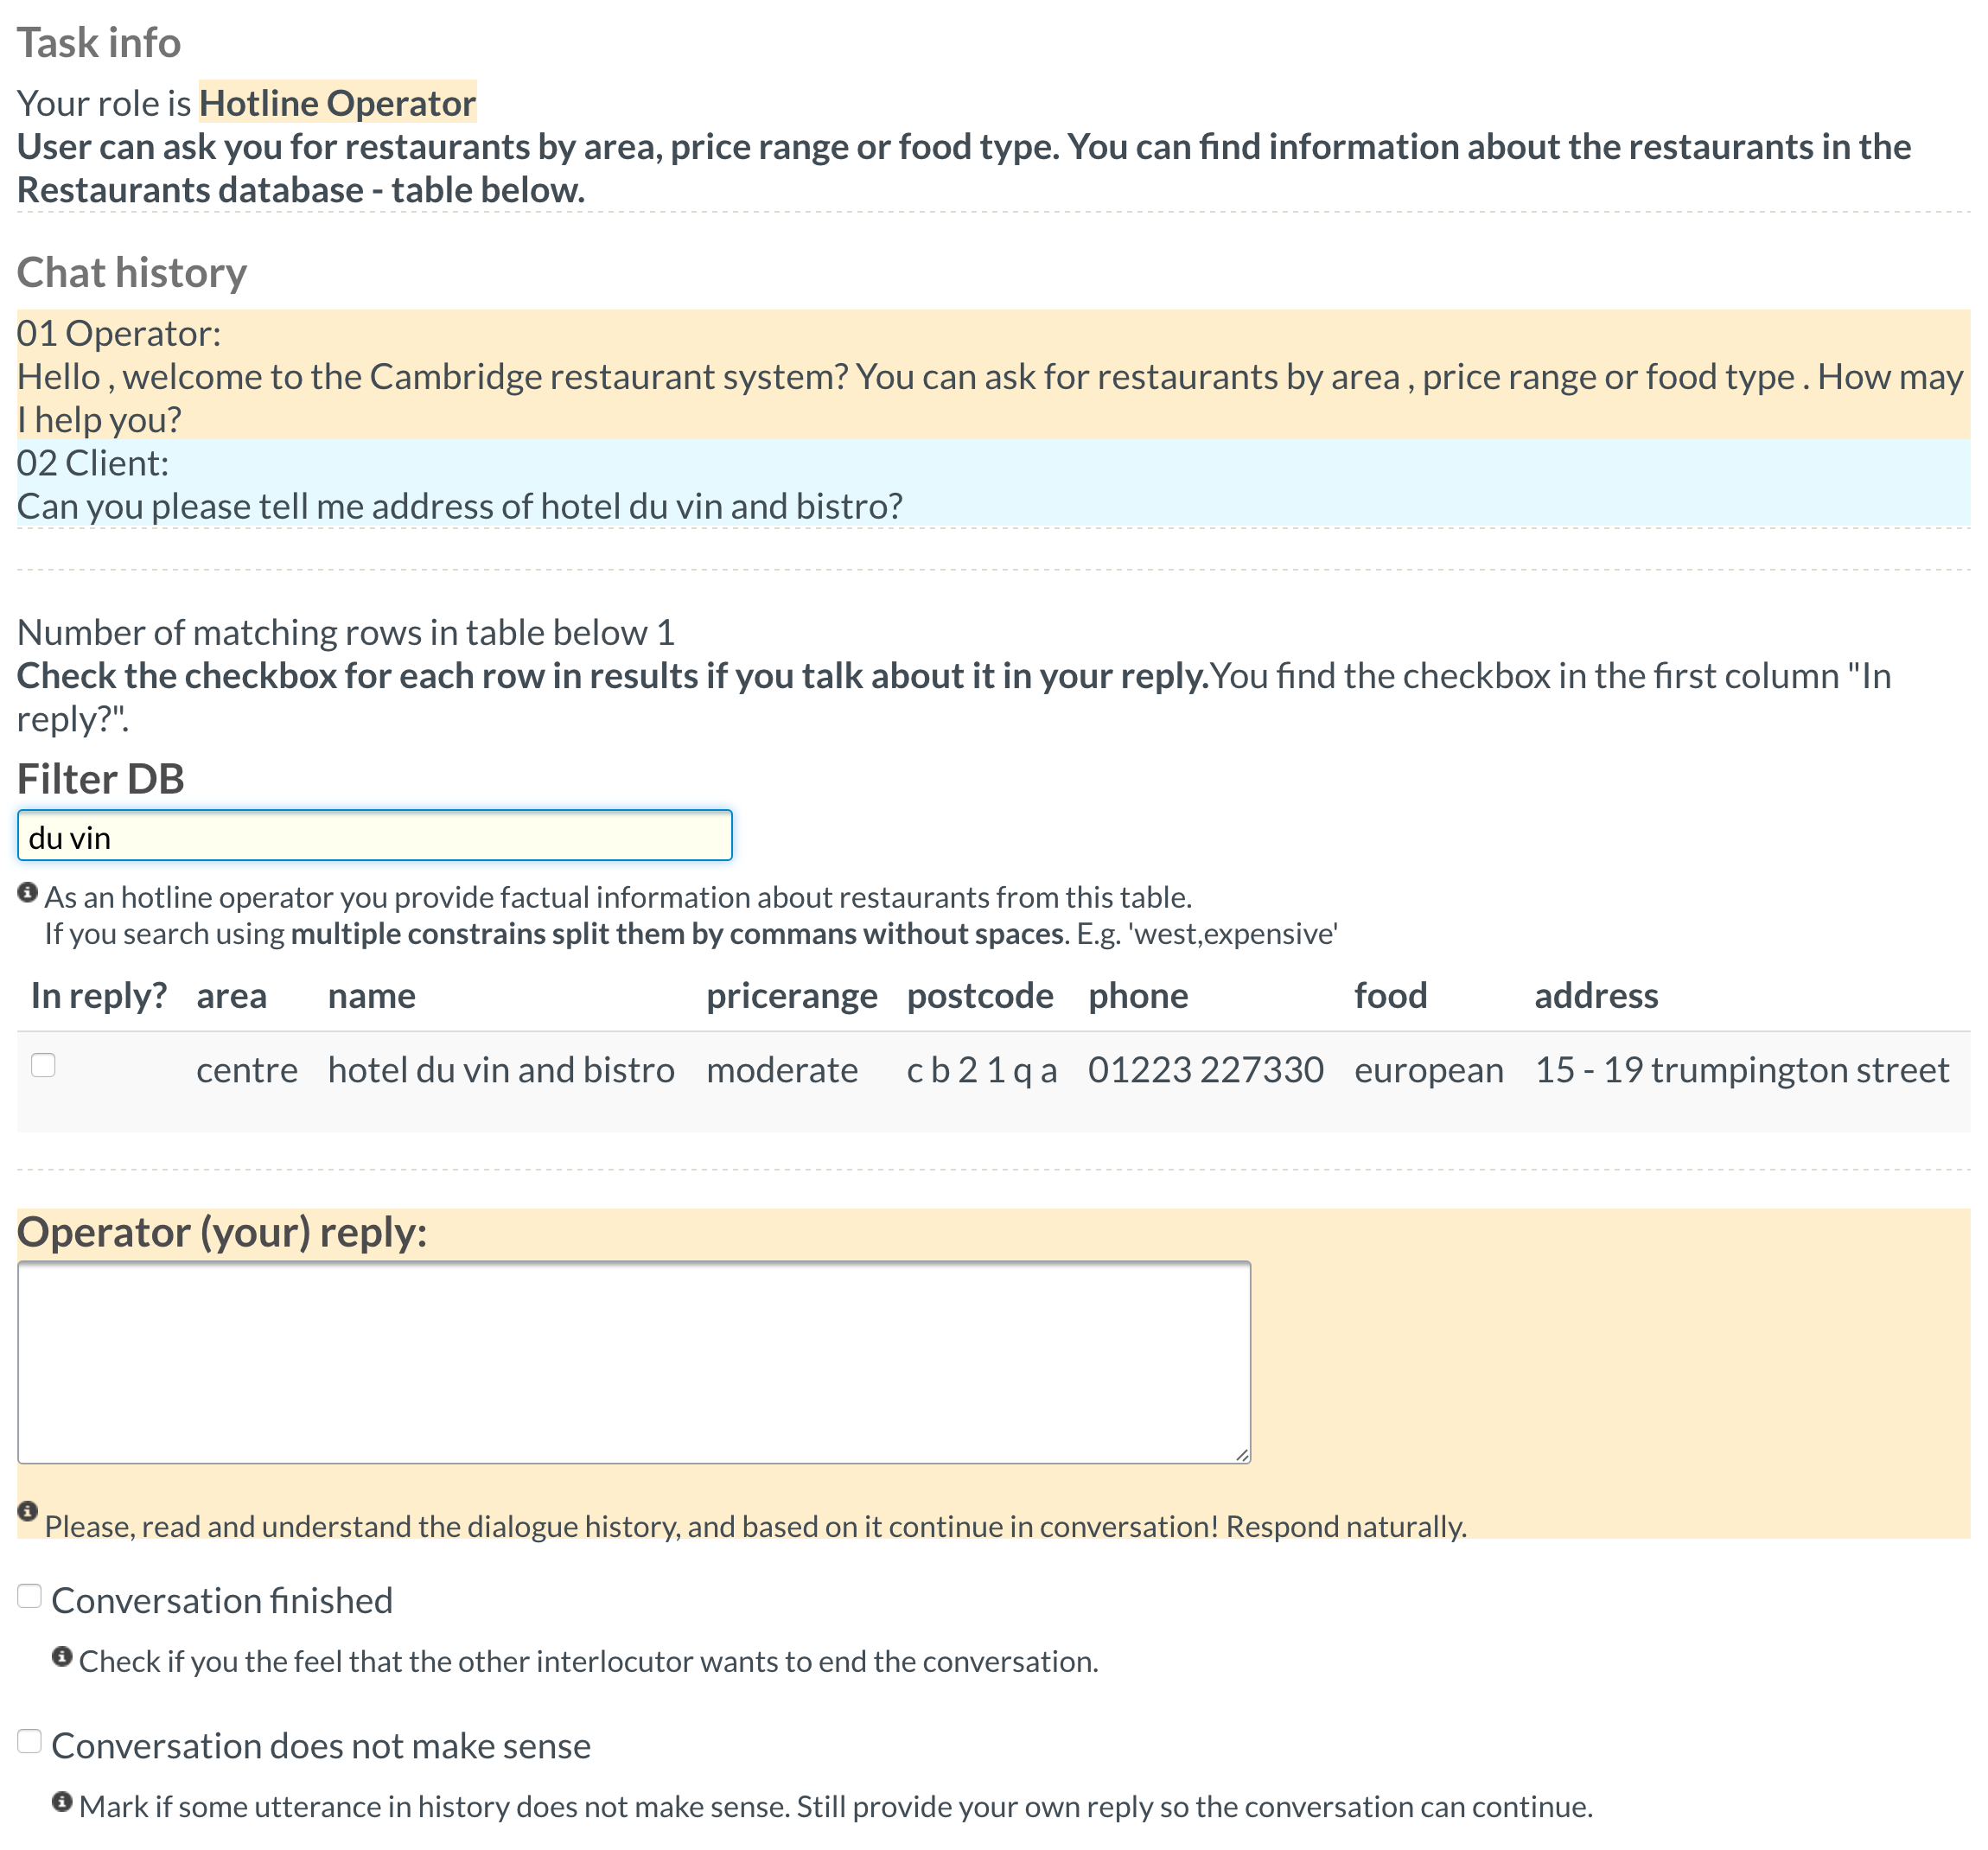
\includegraphics[width=1.0\linewidth]{gui-annotators-system}
    \caption{End-to-end system data collection interface}
    \label{fig:wochat}
\end{figure*}

\subsubsection*{Data augmentation through exploration}
The last of the planned experiments investigates if our implementation of error recovery detection and our clarification strategies are robust enough to label and thus discover new valid actions for given dialogue history.
The idea key idea behind the experiment say that in narrow domain task oriented system the dialogues tend to be repetitive.
The repetitiveness may not seem natural for regular users, but mainly it proves to the system that if conversations after given history tend to continue\footnote{Without detected misunderstanding.} the system performs well.
We want to use such conversations where the system has reasonable confidence of its action to intentionally slightly change the system reply.
If we not detect misunderstanding in several cases of such new reply for given context, we will suppose we can include it as new data point. 
The new data points - conversations - will be added to original dataset.
We suppose that we want to improve a end-to-end systems trained from conversational data such as described at Section~\ref{sec:e2end}.
The system is able to produce alternatives for each predicted actions and also their confidence scores.
Using the scores we may not choose the recommended action by the system, but our active learning algorithm will decide on the alternative.
We will use coverage and precision of problematic situation described in~\cite{meena_datadriven_2016}
\todo{Which framework will we use for suggesting alternatives 1. active learning framework with variables - failure of following dialogue - number of such history context seen - confidence of alternatives?}
% features from Raveesh Thesis 
%  - utterance similarity - cosine distance 
%  - disconfirmation - no/not presenece
%  - corrections arguments for API call changed (is it the same API call?)
%  - change of topic
%       - expected API call in previous turn
%       - number of changed arguments
%       - cosine distance from previous API call
% unweighted average recall
% for each domain experiment how many users need for estimating ground truth reliably


\subsubsection*{Data discovery through misunderstanding}
A special case of misunderstanding which is worth attention is presenting incorrect information from DB to the users.
One example may be missing, outdated or incorrect piece of information in the DB.
Currently, we want to focus only on the incorrectly or outdated information when the user knows the correct answer.
We want to explore if user is able to detect that system answer does not match reality and also if it is able to provide the correct answer.
In this experiment we will use crowd-source workers to correct some intentionally outdated information about restaurant domain in Cambridge.
The interface displays just the dialogue history for the user and also the DB to the operator (see see~Figure~\ref{fig:wochat}).
For this experiment, a user will not be only informed about restaurant using text system reply which may be outdated, but a leaflet with updated address, price range and menu will be presented to the user.
The user will be instructed to tell the system that it is providing incorrect information.
We will investigate how often the user notice the mismatch between the information provided and the true state presented in the leaflet.
Second, we will evaluate how accurately our system is able to detect that user is correcting its information and how the system is able to parse the information from users answers.



\section{Discussion}
\label{sec:discussion}

We see the emerging end-to-end systems~\cite{williams2016end,weston2015endtoend_prereq,wen_networkbased_2016} as big step forward to reducing expert effort needed in building dialogue systems.
However, the human effort put into building even narrow domain task oriented system just shifted from precious expert work to more scalable crowd-source annotators effort~\cite{wen_networkbased_2016,serban_building_2015}.
We present series of experiments which should study how such scalable approach is pushed even further by collecting annotation through interactions.
In addition, the same methods can be used to extracting and updating knowledge from conversations which is almost unexplored direction how to extend dialogue system domain and knowledge.

There is well established research direction of reducing the amount of labeled data needed by inverse reinforcement learning.
The work of~\cite{nouri_cultural_2012} shows that.
More recently,~\cite{su2016active} described active reward learning using unsupervised neural network embeddings and Gaussian processes and managed greatly reduced the amount of data to deploy a system.
The problem with active reward learning of particular architecture is that when the single neural network architecture deprecates the new system can use all the knowledge stored in the system parameters in a very limited way.
Effectively, it means that only the same starting labeled data together with collected unlabeled data can be used for training new architectures. 
We see that collecting annotation have bigger benefit from longer point of view and additionally it is completely orthogonal to active reward learning.

The topics of error detection and error recovery of dialogue systems has been described from several point of view, but we learned that most of experiments focused on ASR errors~\cite{skantze_error_2007}.
The work of~\cite{meena_datadriven_2016} analysed how to detect and recover also from SLU and DM errors.
\todo{Read and include work of~\cite{lopesspedial}.}
However, the work primarily focused to discover errors offline and recommend designers which part of dialogues system needs more attention.

The work of~\cite{pappu_knowledge_2014} detects errors over multiple components over multiple components and then employs post processing step.
This attitude is no longer necessary because all our components are optimized jointly.
However, the work shows interesting insights what might be the most common errors and also further uses error discovery for knowledge acquisition.
The authors report interesting results especially on acquiring missing named entities and enriching the system knowledge base.

In our work, we want to follow up on their results, integrate our strategies to fully trainable system and the most importantly not only learn new facts to directly used in following conversation with user but act as annotations for improving the system itself after retraining.
To our knowledge no other work described a dialog system stores user reward signal in explicit form, aka annotations, for its later optimization.
We would like to investigate its usefulness and compare it with current promising approaches active reward learning~\cite{su2016active} and 
zero-shot learning~\cite{vinyals_matching_2016} which are possible approaches how to exploit users immediate feedback.
Active reward learning tries to induce better latent representation for capturing the reward so the reward is more easily extracted from the dialogue history.
The zero-shot learning applies encoded prior information to extremely efficiently use few data samples provided in the user feedback.


\section{Conclusion}
\label{sec:conclusion}
We presented our work in progress, motivated our past and future experiments and discussed possible difficulties.
Our experiments are mainly described as classification tasks where neural network statistical models will be used.
We choose neural networks because they rather efficiently exploit labeled data but can be also fine-tuned with reinforcement retraining.
However, our goal is to develop strategies which will help a conversational agent collect annotations and facts useful to any statistical inference algorithm.

\section*{Acknowledgments}
This research was partly funded by the Ministry of Education, Youth and Sports of the Czech Republic under the grant agreement LK11221, core research funding, grant GAUK 1915/2015, and also partially supported by SVV project number 260 333. 
We gratefully acknowledge the support of NVIDIA Corporation with the donation of the Tesla K40c GPU used for this research.
Computational resources were provided by the CESNET LM2015042 and the CERIT Scientific Cloud LM2015085, provided under the programme ``Projects of Large Research, Development, and Innovations Infrastructures''.

\bibliographystyle{acl2016}
\bibliography{literature}

\end{document}
